\documentclass[12pt ,a4paper]{exam}
\usepackage[utf8]{inputenc}
\usepackage{amsmath}
\usepackage{amsfonts}
\usepackage{amssymb}
\usepackage{graphicx}

\newcommand\textbox[1]{%
	\parbox{.333\textwidth}{#1}%
}

% Customised items
\usepackage[shortlabels]{enumitem}

% Times New Roman
\usepackage[T1]{fontenc}
\usepackage{newtxmath,newtxtext}

% Code
\usepackage{courier} %% Sets font for listing as Courier.
\usepackage{listings, xcolor}
\lstset{
	tabsize = 4, %% set tab space width
	showstringspaces = false, %% prevent space marking in strings, string is defined as the text that is generally printed directly to the console
	numbers = left, %% display line numbers on the left
	commentstyle = \color{red}, %% set comment color
	keywordstyle = \color{blue}, %% set keyword color
	stringstyle = \color{red}, %% set string color
	rulecolor = \color{black}, %% set frame color to avoid being affected by text color
	basicstyle = \small \ttfamily , %% set listing font and size
	breaklines = true, %% enable line breaking
	numberstyle = \tiny,
}


% Page Setup
\usepackage[a4paper,
bindingoffset=0.2in,%
left=0.5in,
right=0.5in,
top=1in,
bottom=1in,%
footskip=.25in]{geometry}

\author{Yonten Jamtsho}
\begin{document}
	% Title
	\begin{center}
		\textbf{ROYAL UNIVERSITY OF BHUTAN} \\
		\textbf{GYALPOZHING COLLEGE OF INFORMATION TECHNOLOGY} \\
		\textbf{GYALPOZHING : BHUTAN}
	\end{center}
	
	\vspace{0.2cm}
	
	\begin{center}
		%\textbf{SEMESTER END EXAMINATION (AUTUMN 2020)}
		\textbf{SEMESTER END EXAMINATION (AUTUMN 2020)}
	\end{center}
	
	\vspace{0.1cm}
	
	\begin{tabbing}
		\textbf{Class} \=  \hspace{2cm} :  \hspace{0.3cm} \textbf{Bachelor of Science in Information Technology (Year II, Semester I)}     \\ \\
		
		\textbf{Module Title} \hspace{0.65cm} : \hspace{0.3cm} \textbf{Algorithms and Data Structures}       \\ \\
		
		\textbf{Module Code} \hspace{0.55cm} :     \hspace{0.3cm} \textbf{ITS202}     \\ \\
		
		\textbf{Serial No.} \hspace{1.13cm} :       \hspace{0.3cm} \textbf{BSc(IT)/2020/III/F/ITS202/I}          \\ \\
		
		\textbf{Max. Marks} \hspace{0.75cm} :     \hspace{0.3cm} \textbf{50}             \\ \\
		
		\textbf{Max. Time} \hspace{1.04cm} :        \hspace{0.3cm} \textbf{3 Hours}             \\ \\
	\end{tabbing}
	
	\textbf{General Instructions:}
	\begin{enumerate}
		\itemsep0em 
		\item Question paper has written component.
		\item In no circumstances may you remove Answer Books, used or unused, from the Examination Room.
		\item If the answer book is torn or folded or without Exam Cell’s seal, report the matter to the Invigilator and get a new one.
		\item Enter the required details such as Reg.  Number, Module and other information as prescribed.
		\item Do not write your name on any part of the Answer Book.
		\item Number your answer according to the number assigned in the Question Paper.
		\item Do not skip any pages when writing answers.  Any rough sketches/calculations must be shown on the same page.
		\item Do not fold or tear off any pages from the Answer Book. Any answer crossed by you will not be evaluated.
		\item You may request for the supplementary Answer sheets only after the main answer Book is completely used.
		\item A candidate who is found to have unauthorised materials in his /her possession, copying, talking or exchanging any material with others will be dealt with as per the Wheel of Academic Law.
		\item No paper other than Admit Card will be allowed in the Examination Hall/Room unless otherwise specified in the Question Paper.
	\end{enumerate}
	\pagebreak
	
	% Part A title
	\begin{center}
		\noindent \textbf{PART - I} \textbf{ [10 Marks]}\\
		\noindent \textit{Answer all the questions} 
	\end{center}
	
	% Keep space between PAT A and MCQ
	\vspace{0.5cm}
	
	% MQC Title
	\noindent \textbf{Multiple Choice Questions} \hfill \textbf{[10 x 0.5 = 5]}
	
	% Begin your question with customized numbered list
	\begin{enumerate}[start=1,label={\bfseries Q\arabic*)}]
		% Reduce the space between items
		\itemsep0.2em
		 \item How many times can you tear a phonebook with 128 pages (i.e., sheets of paper) in half, each time throwing away one of the halves, before only one page remains?
		\item[] 
		\begin{oneparchoices}
			\choice 6% \hspace is used to keep space between choice
			\choice 7
			\choice 10
			\choice 64
		\end{oneparchoices}
		\item Which strategy returns index of node’s left child in heap where i is the position of a node.
		\item[] 
		\begin{oneparchoices}
			\choice 2i  % \hspace is used to keep space between choice
			\choice 2i + 1 
			\choice i
			\choice i/2
		\end{oneparchoices}
		
		\item Which of the following is false about a binary search tree?
		\item[] 
		\begin{oneparchoices}
			\choice The left child is always lesser than its parent \\ % \hspace is used to keep space between choice
			\choice The right child is always greater than its parent \\
			\choice The left and right sub-trees should also be binary search trees\\
			\choice In order sequence gives decreasing order of elements
		\end{oneparchoices}
	
		\item  Why we need to a binary tree which is height balanced?
		\item[] 
		\begin{oneparchoices}
			\choice to avoid formation of skew trees\\  % \hspace is used to keep space between choice
	    	\choice to save memory \\
	    	\choice to attain faster memory access\\
	    	\choice to simplify storing
		\end{oneparchoices}
	
		\item If several elements are competing for the same bucket in the hash table, what is it called?
		\item[] 
		\begin{oneparchoices}
			\choice  Diffusion\\% \hspace is used to keep space between choice
			\choice  Replication\\
			\choice Collision\\
			\choice Duplication
	 	\end{oneparchoices}
 	    
 	   	\item The worst case time complexity of BST is
 	    \item[] 
 	    \begin{oneparchoices}
 	    	\choice  O(n)\\% \hspace is used to keep space between choice
 	    	\choice  O(log n)\\
 	    	\choice O(n log n)\\
 	    	\choice O($n^2$)
 	    \end{oneparchoices}
 		\item A simple method for sorting that is effective whenever the keys are small integers.
     	\item[]   
     	 \begin{oneparchoices}
     		\choice  Key Indexed Counting\\% \hspace is used to keep space between choice
     		\choice  Shell Sort\\
     		\choice Merge Sort\\
     		\choice Insertion Sort
     	\end{oneparchoices}
     
     \item Sorting algorithms which loops through till n-2 is
     \item[]   
     \begin{oneparchoices}
     	\choice  LSD Sort\\% \hspace is used to keep space between choice
     	\choice  Quick Sortt\\
     	\choice Bubble Sort\\
     	\choice Heap Sort
     \end{oneparchoices}
 
    \item ....... Is the Example of Symbol Table.
    \item[]   
    \begin{oneparchoices}
    	\choice  Strings\\% \hspace is used to keep space between choice
    	\choice  BSc in IT programme\\
    	\choice Book\\
    	\choice DNS Lookup
    \end{oneparchoices}
    
    \item Consider the following operation performed on a stack of size 5.
    Push(1);\\
    Pop();\\
    Push(2);\\
    Push(3);\\
    Pop();\\
    Push(4);\\
    Pop();\\
    Pop();\\
    Push(5);\\
    
    \item []After the completion of all operation, the no of element present on stack are
    \item[]   
    \begin{oneparchoices}
    	\choice  1\\% \hspace is used to keep space between choice
    	\choice  2\\
    	\choice 3\\
    	\choice 4
    \end{oneparchoices}
 
    \end{enumerate}
	
	\noindent \textbf{Fill in the blanks} \hfill\textbf{ [5 x 0.5 = 2.5]}
	
	% Continue the items from 2
	\begin{enumerate}[start=11,label={\bfseries Q\arabic*)}]
		\item   .................. Binary Tree require more memory space.
		\item ........... sorts strings which are  of same length.
		\item ...............  is a directed cycle whose sum of edge weights is negative.
		\item A minimum spanning tree has ............. edges where V is the number of vertices in the given graph.
		\item Worst-case time complexity is also known as .........
	\end{enumerate}
	
	\noindent \textbf{True or False} \hfill\textbf{ [5 x 0.5 = 2.5]}
	
	% Continue the items from 2
	\begin{enumerate}[start=16,label={\bfseries Q\arabic*)}]
		\item A stack is a first-in, first-out data structure.
		\item Full BT is a strictly binary tree with all leaves in the last level.
		\item Individual elements in linked list are stored in consecutive memory location.
		\item The worst case time complexity of the insert operation into an AVL tree is O(log n), where n is the number of nodes in the tree.
		\item Heap is sorted in nature.
		
	\end{enumerate}
	\vspace{0.1mm}
	\pagebreak
	% Part B title
	\begin{center}
		\textbf{PART - II} \textbf{[15 Marks]}\\
		\noindent \textit{SHORT ANSWER QUESTION} \\
		\noindent \textit{Answer all the questions} 
	\end{center}

	\begin{enumerate}[start=1,label={\bfseries Q\arabic*)}]
		\item Complete the table below by specifying lower ($\omega$) and upper (O) bounds for each algorithm. Assume that the input to each algorithm is an array of size n.  \hfill \textbf{ [0.5 * 5 = 2.5]}
		
		\begin{table}[h]
			\centering
			\begin{tabular}{|l|l|l|l}
				\cline{1-3}
				\textbf{Algorithms} & \textbf{$\omega$} & \textbf{O}  &  \\ \cline{1-3}
				Binary Search &   &     &  \\ \cline{1-3}
				Bubble Sort&   &     &  \\ \cline{1-3}
				Linear Search&   &     &  \\ \cline{1-3}
				Merge Sort&    &     &  \\ \cline{1-3}
				Selection Sort &   &     &  \\ \cline{1-3}
			\end{tabular}
		\end{table}
		\item What does it mean if some algorithm is in $\theta$ (n)? Give example or scenerio of such time complexity. \hfill \textbf{[1.5]}
		\item What are the two data structure used in finding SPT(Shortest Path Problem) \hfill \textbf{[1]}
		\item Explain Hibbard Deletion of BST with the help of example. \hfill \textbf{[3]}
	    \item For the tree given below, find the preorder, inorder and postorder traversal. \hfill \textbf{[3]}
	    \begin{figure} [h]
	    	\centering
	    	\includegraphics[width=0.4\linewidth]{"Screenshot 2020-12-26 at 9.29.16 AM"}
	    	\caption{Tree}
	    	\label{fig:screenshot-2020-12-26-at-9}
	    \end{figure}
	     \item Explain four Operation of Linked List with the help of diagram. \hfill \textbf{[4]}
	   
	\end{enumerate}
	\pagebreak
	% Part C title
	\begin{center}
		\textbf{PART - III} \textbf{[25 Marks]}\\
		\noindent \textit{LONG ANSWER QUESTIONS} \\
		\noindent \textit{Answer all the questions}  
	\end{center}
	
	\begin{enumerate}[start=1,label={\bfseries Q\arabic*)}]
	\item Appply shell sort on the given String \hfill\textbf{[5]} 
	\item [] E A S Y S H E L L S O R T Q U E S T I O N
	
	\item Paro Airport runaway reservation system have only one runway available. Following details are provided for reservation. 
	\begin{itemize}
		\item Reserve request: specifies landing time t.
		\item Add t to the set R of landing times if no other landings are
		scheduled within k minutes.
		\item k can vary: let’s assume it is statically set (e.g. 3 min). 
		\item After landing, remove request from R.
		\item What operations do we need in the data structure?
			\begin{itemize}
				\item Adding requests. If they satisfy constraint!
				\item Removing requests.
				\item Notion of time, checks every m seconds to update the structure.
				\item Nutshell: we need a data structure that allows for insertion and removal of elements.
				\item Additional requirement: operations in O(lg n)
			\end{itemize}
	\end{itemize}
	\item [] List and Explain with diagram all the data structure available comparing interms of their time complexity and finally suggest the best data structure to opt for given you are the developer of this system.  \hfill\textbf{[5]}
	\item Show the AVL tree that results after each of the integer keys \textcolor{blue}{ 9, 27, 50, 15, 2, 21, and 36} are inserted, in that order, into an initially empty AVL tree. Clearly show the tree that results after each insertion, and make clear any rotations that must be performed.\hfill\textbf{[5]} 
	\item Find the minimum spanning tree using Kruskal’s algorithm and provide the overall weight of the MST for the given figure 2.\hfill\textbf{[5]}
	\item []
	\begin{figure}[h]
		\centering
		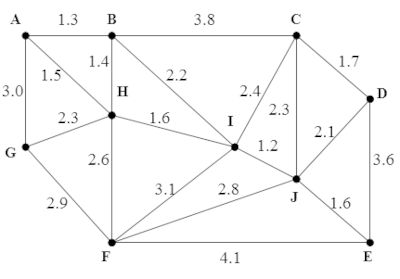
\includegraphics[width=0.6\linewidth]{L2FwcGhvc3RpbmdfcHJvZC9ibG9icy9BRW5CMlVvRjE0bjJhd2cyaXNleU4ybUhLZWxBSDlaQlBzX3Z6NjZONXEzMmFQZTdaQ2cwVlFOQWozdHNBNWdXemFIXzhxSXhwcU1lRDFIbnlDeHJNUGZzSVZpTW4zeDhpdy5idmJfeUlpOVkyNlVLSEdi_400_400}
		\caption{Graph}
		\label{fig:l2fwcghvc3rpbmdfchjvzc9ibg9icy9brw5cmlvvrje0bjjhd2cyaxnleu4ybuhlzwxbsdlaqlbzx3z6njzonxezmmfqztdaq2cwvlfoqwozdhnbnwdxemfixzhxsxhwcu1lrdfibnldehjnugzzsvzptw4zedhpdy5idmjfeulpovkynlvlsedi400400}
	\end{figure}
	\pagebreak
	\item Perform DFS on the graph given.\hfill\textbf{[5]} 
	\begin{figure}[h]
		\centering
		\includegraphics[width=1\linewidth]{"Screenshot 2020-12-27 at 8.15.57 PM"}
		\caption{Graph:DFS}
		\label{fig:screenshot-2020-12-27-at-8}
	\end{figure}
	


	\end{enumerate}
		$------------ ------BEST WISHES----------------------------$
\end{document}